%%%%%%%%%%%%%%%%%%%%%%% file template.tex %%%%%%%%%%%%%%%%%%%%%%%%%
%
% This is a template file for Web of Conferences Journal
%
% Copy it to a new file with a new name and use it as the basis
% for your article
%
%%%%%%%%%%%%%%%%%%%%%%%%%% EDP Science %%%%%%%%%%%%%%%%%%%%%%%%%%%%
%
%%%\documentclass[option]{webofc}
%%% "twocolumn" for typesetting an article in two columns format (default one column)
%
\documentclass{webofc}
\usepackage[varg]{txfonts}   % Web of Conferences font
%
% Put here some packages required or/and some personnal commands
%
%
\begin{document}
%
\title{Continuous Performance Benchmarking Framework for ROOT}
%
% subtitle is optionnal
%
%%%\subtitle{Do you have a subtitle?\\ If so, write it here}

\author{\firstname{Brian Paul} \lastname{Bockelman}\inst{1}\fnsep\thanks{\email{bbockelm@cse.unl.edu}} \and
        \firstname{Oksana} \lastname{Shadura}\inst{1}\fnsep\thanks{\email{oksana.shadura@cern.ch}} \and
        \firstname{Vassil} \lastname{Vassilev}\inst{2}\fnsep\thanks{\email{vasil.georgiev.vasilev@cern.ch}}
        % etc.
}

\institute{University of Nebraska Lincoln, 1400 R St, Lincoln, NE 68588, United States
\and
           Princeton University, Princeton, New Jersey 08544, United States
          }

\abstract{%
  

Foundational software libraries such as ROOT are under intense pressure to avoid software regression, including performance regressions. Continuous performance benchmarking, as a part of continuous integration and other code quality testing, is an industry best-practice to understand how the performance of a software product evolves over time. We present a framework, built from industry best practices and tools, to help to understand ROOT code performance and monitor the efficiency of the code for a several processor architectures. It additionally allows historical performance measurements for ROOT I/O, vectorization and parallelization sub-systems.

We utilize the Google benchmarking library to execute micro benchmarks of selected hotspot functions in ROOT and related libraries. This provides detailed data measurements, including memory usage and CPU instruction counters. Additionally, the framework manages traditional benchmarking pitfalls via repeating unstable benchmarks and providing a stable performance environment over time. The performance data points from continuous benchmarking are fed into an InfluxDB database and provided to the developer community via a Grafana-based dashboard. This performance benchmarking framework, built on generic and flexible infrastructure, is meant to be reusable by other projects.

}
%
\maketitle
%
\section{Introduction}
\label{intro}

\section{Motivation}
Foundational software libraries such as ROOT are under intense pressure to avoid software regression, including performance regressions. Continuous performance benchmarking, as a part of continuous integration and other code quality testing, is an industry best-practice}} to understand how the performance of a software product evolves over time. We present a framework, built from industry best practices and tools, to help to understand ROOT code performance and monitor the efficiency of the code for a several processor architectures. It additionally allows historical performance measurements for ROOT I/O, vectorization and parallelization sub-systems.

\section{Project Goals}
We aim to provide:
\begin{enumerate}
\item Continuous performance monitoring of ROOT components;
\item Speculative performance monitoring on opened pull requests (PR);
\item Rich and customizable visualizations to aid performance analysis.
\end{enumerate}

\begin{block}{Implementation}
We utilize the Google benchmarking library\cite{gbench}}to execute micro benchmarks of selected hotspot functions in ROOT and related libraries. This provides detailed data measurements, including memory usage and CPU instruction counters. Additionally, the framework manages traditional benchmarking pitfalls via repeating unstable benchmarks and providing a stable performance environment over time. The performance data points from continuous benchmarking are fed into an InfluxDB database and provided to the developer community via a Grafana-based dashboard.} This performance benchmarking framework, built on generic and flexible infrastructure, is meant to be reusable by other projects. The tool can be connected to Jenkins or other similar services as shown in Fig~\ref{fig:InformationFlow}.

\begin{figure}
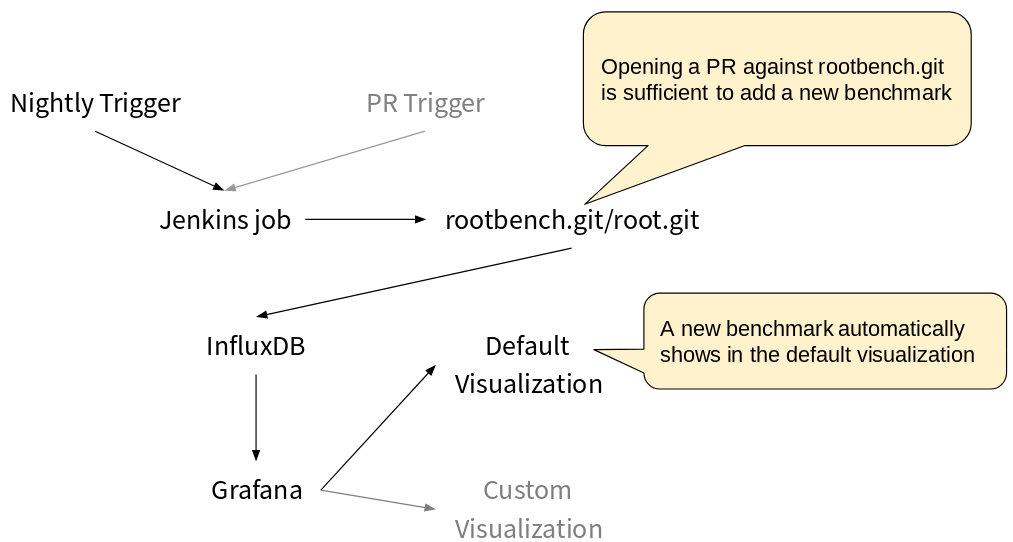
\includegraphics[width=1.0\linewidth]{pictures/flow.png}
\caption{Jenkins -- ROOTBench Flow.}
\label{fig:InformationFlow}
\end{figure}

\section{Results}
We have defined a basic set of measurements: Real Time (RT); CPU Time and RSS memory footprint}. The set of performance indicators could be expanded with custom ones. Google Benchmark enables multi-threading analyses and addition of custom parameters such as number of branches in a generated TTree.

\begin{figure}
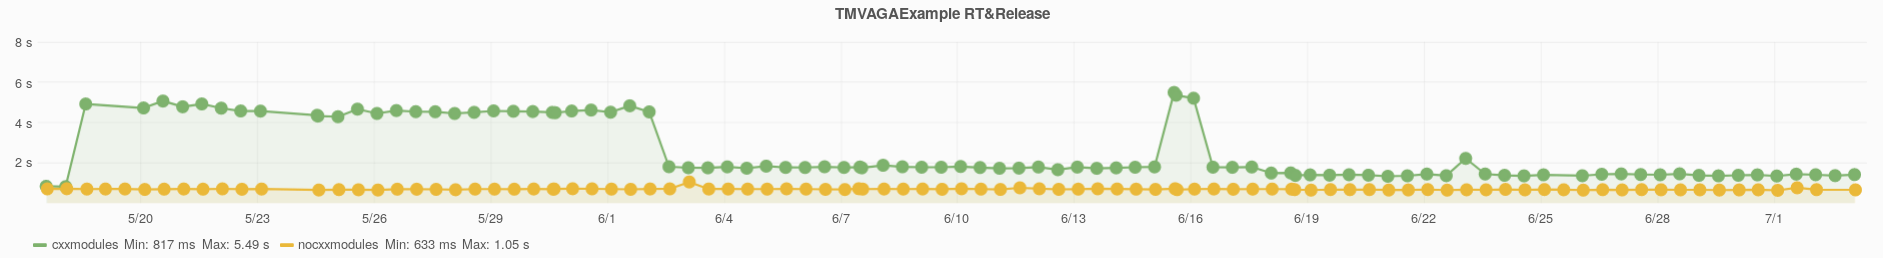
\includegraphics[width=1.0\linewidth]{pictures/1.png}
\caption{Performance improvements (enhancements in runtime) in Interpreter benchmarks}
\label{interp}
\end{figure}

\begin{figure}
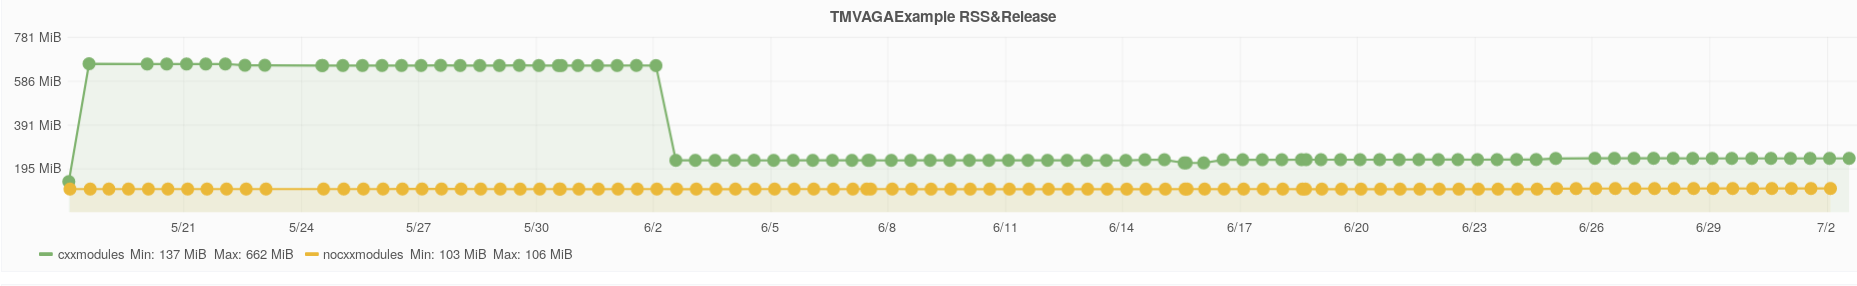
\includegraphics[width=1.0\linewidth]{pictures/2.png}
\caption{Memory Footprint Comparison Between ROOT runtime\_cxxmodules and pch Features}
\label{interp1}
\end{figure}

\begin{figure}
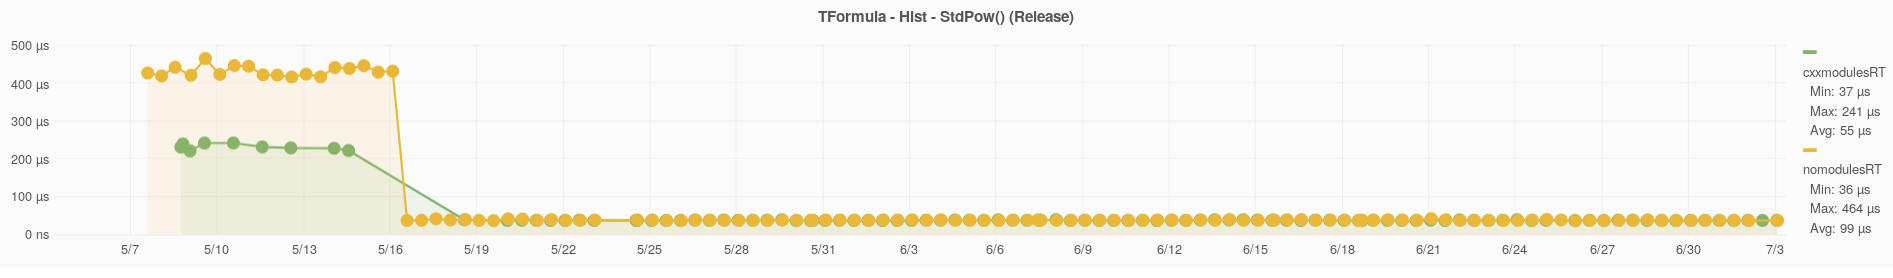
\includegraphics[width=1.0\linewidth]{pictures/4.png}
\caption{TFormula Speedup.}
\label{tform}
\end{figure}

\begin{figure}
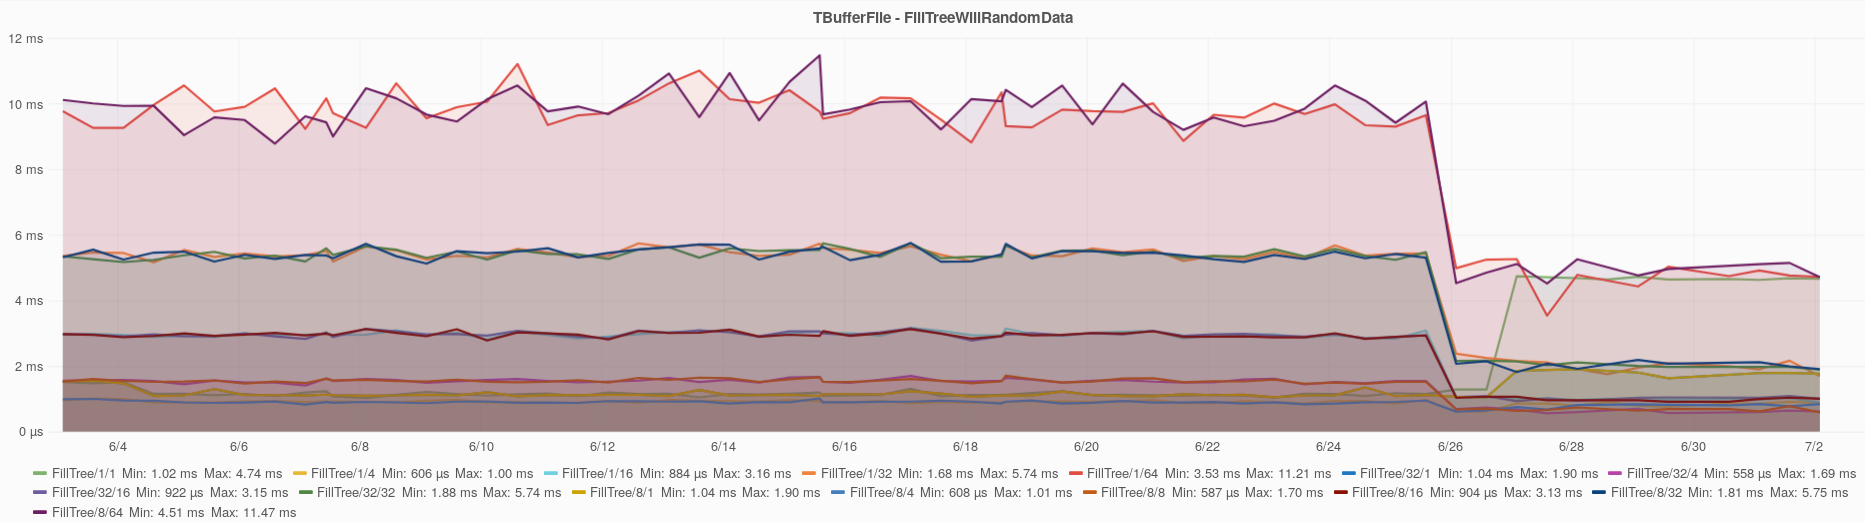
\includegraphics[width=1.0\linewidth]{pictures/5.png}
\caption{Threading Improvements in TBufferMerger}
\label{tbuf}
\end{figure}

\begin{figure}
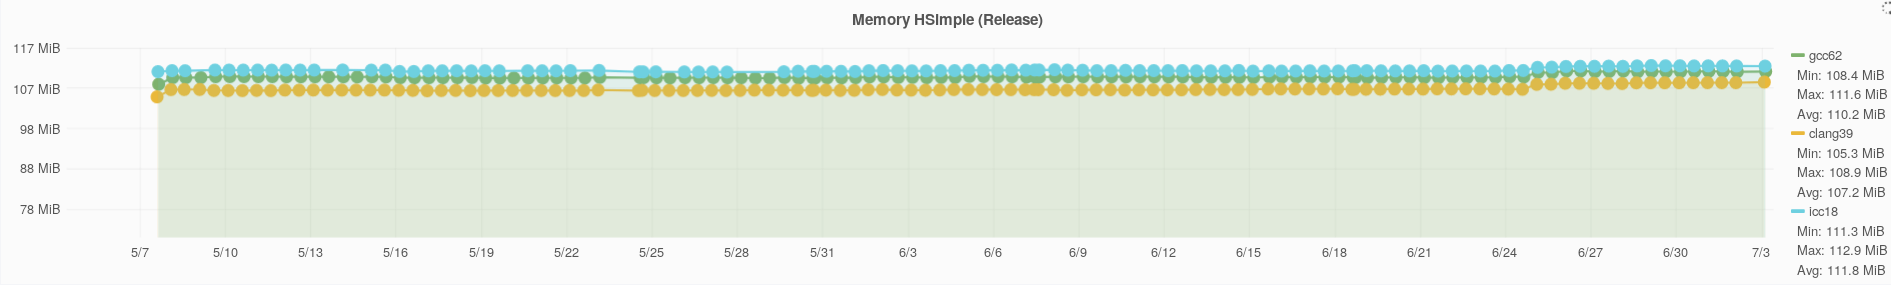
\includegraphics[width=1.0\linewidth]{pictures/7.png}
\caption{Memory Footprint of clang-, icc- and gcc-compiled ROOT Running HSimple}
\label{fig:compilers}
\end{figure}

\begin{figure}
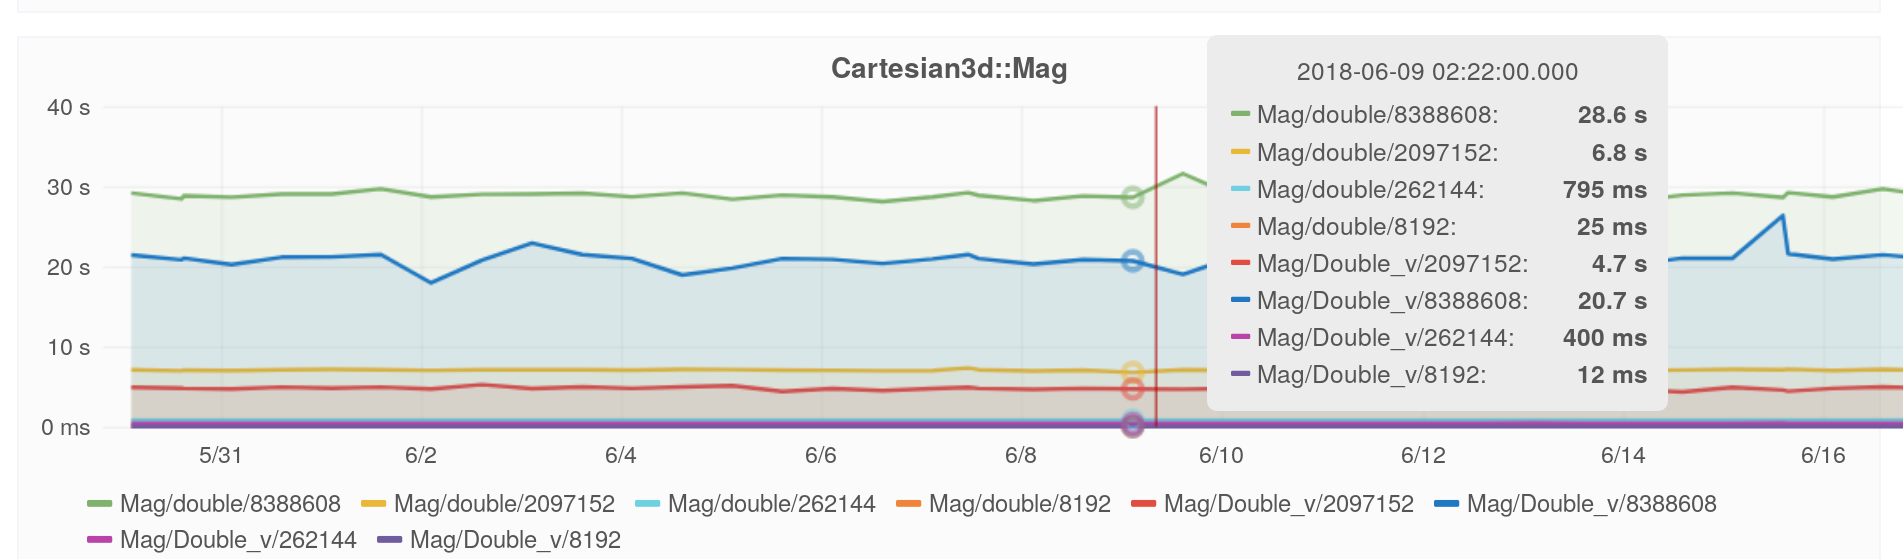
\includegraphics[width=1.0\linewidth]{pictures/genvector.png}
\caption{RT comparison of vectorized and scalar code in GenVector::Mag()}
\label{fig:genvec}
\end{figure}

Fig 2-7 show several real-world examples:
\begin{itemize}
\item Interpreter -- implementation of Bloom filter as per \href{https://github.com/root-project/root/pull/2093}{PR2093}, \href{https://github.com/root-project/root/pull/2137}{PR2137} and \href{https://github.com/root-project/root/pull/2204}{PR2204} (Fig\,\ref{interp1})
\item TFormula -- remove debug check in TFormula as per from \href{https://github.com/root-project/root/pull/2017}{PR2017} (Fig.\,\ref{tform})
\item TBufferMerger -- remove callback functionality to avoid over subscription of the machines as per \href{https://github.com/root-project/root/pull/2245}{PR2245}  (Fig.\,\ref{tbuf})
\item Hsimple benchmark -- comparison of memory footprint of ROOT compiled with different compilers (Fig \ref{fig:compilers})
\item GenVector -- comparison of scalar and vectorized implementation in GenVector library (Fig. \ref{fig:genvec})
\end{itemize}

\section{Conclusion}
The prototype is very functional and it has been often used to find performance degradation. Performance sensitive code can be monitored at the cost of a standard pull requests against the ROOTbench GitHub repository. Several external benchmarking contributions have been submitted some of them track TMVA and RDF components. We have enumerated several important future improvements:
\begin{itemize}
\item Enable the current infrastructure to work on pull requests (PR);
\item Introduce alerts if metrics have gone beyond defined thresholds;
\item Complement performance graphs with performance flame graphs;
\item Introduce more benchmarks statistics to stabilize the RT metrics;
\item Introduce performance node monitoring to monitor regressions in the host hardware to reduce noise;
\item Implement versioning of dashboards (dashboards auto generation via JS).

\end{itemize}

Performance of large-scale systems is fragile and can vary on the different systems. It is vital for the projects to offer a set of tools and benchmarks allowing coders to reason about performance. We hope ROOTBench is a step towards recognizing and solving the problem ensuring better sustainability of HEP Software.


\begin{thebibliography}{}
%
% and use \bibitem to create references.
%
\bibitem{RefJ}
% Format for Journal Reference
Journal Author, Journal \textbf{Volume}, page numbers (year)
% Format for books
\bibitem{RefB}
Book Author, \textit{Book title} (Publisher, place, year) page numbers
% etc
\end{thebibliography}

\end{document}

% end of file template.tex

<div id='footer'><table width='100%'><tr><td class='right'><a href='http://fusioninventory.org/'><span class='copyright'>FusionInventory 9.1+1.0 | copyleft <img src='/glpi/plugins/fusioninventory/pics/copyleft.png'/>  2010-2016 by FusionInventory Team</span></a></td></tr></table></div>